%!TEX root = ../bachelor.tex
\chapter{Einleitung}
\todo{einleitung schreiben}
\begin{itemize}
	\item nur eine Kamera statt 5
	\item zur Beobachtung von Drosophila melanogaster - Larven
	\item stressfreie Umgebung als auf dem FIM-Tisch
	\item kein Stitching mehr notwendig, keine synchronsisation
	\item besseres Verhältnis zwischen Gehege und Kameras
	\item keine Ghosts
	\item Entzerrung bleibt
	\item Larven oben wesentlich größer als unten (perspektivische Verzerrung) $\rightarrow$ kein relativer Vergleich der Größe möglich
	\item Verfolgen von Larven, ändern die Größe $\rightarrow$ auch schlecht
	\item Entzerrungsverfahren, dass die 3D - Kegeloberfläche auf die 2D-Mantelfläche abbildet, sodass ein Vergleich möglich ist $\rightarrow$ Thema der Arbeit
	\item zwei verschiedene Verfahren werden vorgestellt?
\end{itemize}

\begin{figure}[!htb]
	\centering
	\begin{subfigure}{.5\textwidth}
		\centering
		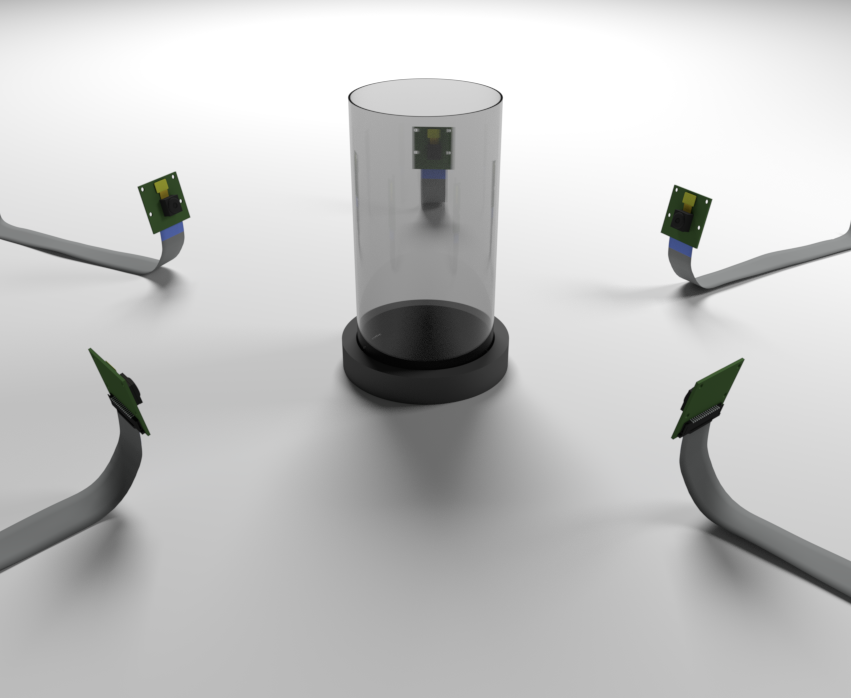
\includegraphics[width=0.95\textwidth]{images/renderCylinder.png}
		\caption{bisheriger Ansatz}
	\end{subfigure}%
	\begin{subfigure}{.5\textwidth}
		\centering
		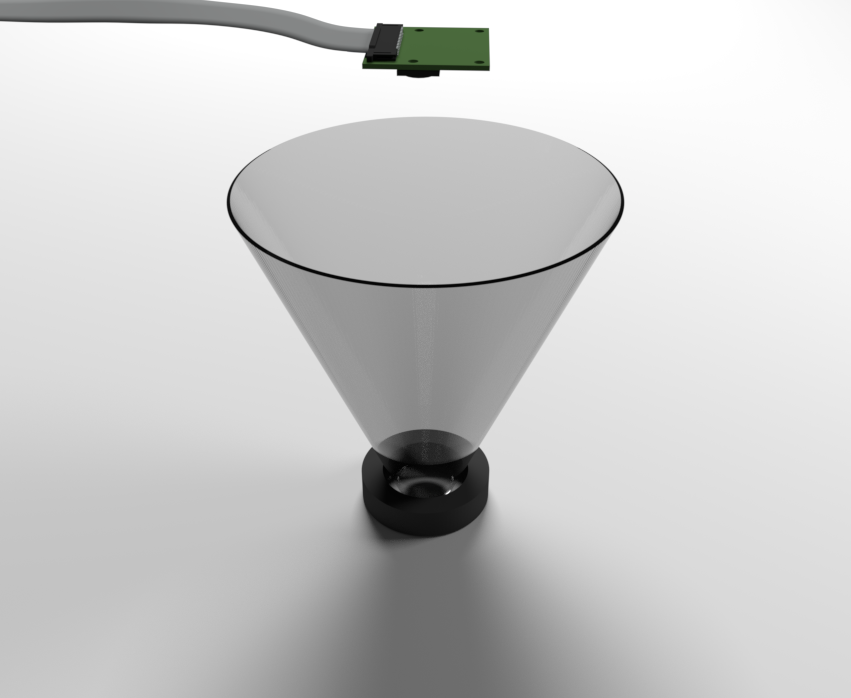
\includegraphics[width=0.95\textwidth]{images/renderCone.png}
		\caption{neuer Ansatz}
	\end{subfigure}
	\caption{beide Ansätze im Vergleich}
	\label{fig:renderedSetup}
\end{figure}